\documentclass{beamer} % [handout] para imprimir eliminando transiciones

%\usefonttheme[onlymath]{serif}
%\usepackage{fontspec}
%\defaultfontfeatures{Mapping=tex-text}
%\setsansfont[Ligatures={Common}]{Futura}
%\setmonofont[Scale=0.8]{Monaco} 

\usepackage{beamerthemesplit}
\usepackage[utf8]{inputenc}
\usepackage[spanish]{babel}
\mode<presentation>
\usetheme{default}
\usecolortheme{dolphin}
\usepackage{alltt}                                    % \begin{alltt}
\usepackage{amssymb}                                  % mathematical symbols
\usepackage{comment}
\usepackage{tabto}                                    % \tabto
\usepackage{tikz}
\usetikzlibrary{automata}
\usetikzlibrary{positioning}
\usetikzlibrary{calc}

\usepackage{verbatim}                                 % comentarios

\title{Lenguajes de Programación}                     %[titulo corto]
\author{Fabián Riquelme Csori}                        %[nombre corto]
\date{2017}                                           %[fecha corta]
\institute{Universidad de Valparaíso}                 %[instituto corto]

\newcommand{\HRule}{\rule{\linewidth}{0.2mm}\\[1ex]}
\newcommand{\blue}[1]{\textcolor{blue}{#1}}
\newcommand{\red}[1]{\textcolor{red}{#1}}
\newcommand{\redb}[1]{{\color{red!70!black}{#1}}}
\newcommand{\green}[1]{{\color{green!70!black}{#1}}}
\newcommand{\gray}[1]{{\color{gray!50!white}{#1}}}
\newcommand{\yell}[1]{{\color{yellow!70!black}{#1}}}
\newcommand{\lQ}{\mbox{``}}
\newcommand{\rQ}{\mbox{''}}
% \alert{texto destacado en rojo}
% \color{green} Color en verde
% \structure{texto en lila}


\begin{document}

%\begin{frame}%[plain]
%  \titlepage
%\end{frame}
%
% [opciones]:
% plain: oculta barra de navegacion, deja + espacio para contenido
% fragile: usar comandos como verbatim
% b,c,t: alineacion vertical
% label=nombre_etiqueta
% allowframebreaks: divide contenido en varios frames si es demasiado largo
% shrink: para escribir mucho texto en una transparencia, reduciendo tamano de fuente

%%%%%%%%%% PORTADA %%%%%%%%%%
\begin{frame}[plain]
  \begin{figure}[h]
    \begin{minipage}{0.3\textwidth}
    
\includegraphics[width=.9\textwidth]{./image/logo-UV.png}
    \end{minipage}
    \begin{minipage}{0.65\textwidth}
     $~$\\[3.6ex]
     \footnotesize{Escuela de Ingeniería Civil Informática}\\
     \footnotesize{Facultad de Ingeniería}
    \end{minipage}
  \end{figure}
  \begin{center}
    \vspace{1ex}
    \HRule
    \Large{Lenguajes de Programación}\\{\small Capítulo V: Nombres, ámbitos y ligados}\\[-1ex]
    \HRule\vspace{1ex}
    \large{Fabián Riquelme Csori}\\[.5ex]\footnotesize{fabian.riquelme@uv.cl}\\[6ex] {\tiny 2017-II}\\[6ex]
  \end{center}
\end{frame}

%%%%%%%%%% INDEX %%%%%%%%%%
\begin{frame}
 \frametitle{Index}
 \scriptsize 			% reducir tamano de letra
 \tableofcontents		%[pausesections]
\end{frame}

%%%%%%%%%%% ACTUAL INDEX %%%%%%%%%%
%\AtBeginSection[] %generar indice automaticamente
%{
%\begin{frame}<beamer>%[plain]
% \frametitle{Index}
% \framesubtitle{subtitulo}
% \scriptsize
% \tableofcontents[currentsection, currentsubsection]
%\end{frame}
%}

%==============================
\section{Asociación de entidades (Name binding)}

%------------------------------
\subsection{Nombres y abstracción}

\begin{frame}{Identificadores}
    
    Formas de representar en SML la fórmula:
    $$\frac{5+4+(2-(3-(6+\frac{4}{5})))}{3(6-2)(2-7)}$$
    \medskip
    
    {\footnotesize 
    \texttt{\redb{val} e = (5.0 + 4.0 + (2.0 - (3.0 - (6.0 + (4.0 / 5.0))))) /}\\
    \texttt{$~~~~~~~~$(3.0 * (6.0 - 2.0) * (2.0 - 7.0))}}
    \bigskip
    
    {\scriptsize 
    \texttt{\redb{val} expr = \redb{let val} num = (5.0 + 4.0 +(2.0 -(3.0 -(6.0 +(4.0 / 5.0)))))}\\
    \texttt{$~~~~~~~~~~~~~~~$\redb{val} den = (3.0 * (6.0 - 2.0) * (2.0 - 7.0))}\\
    \texttt{$~~~~~~~~~~~$\redb{in} num / den}\\
    \texttt{$~~~~~~~~~~~$\redb{end};}
    }\medskip
    
    \url{www.tutorialspoint.com/codingground.htm}
    \pause\smallskip
    
    La segunda versión usa más código, pero introduce \textbf{identificadores} con \redb{\texttt{let}} para mayor legibilidad.
\end{frame}

\begin{frame}{Nombrar y Conquistar}
    \begin{itemize}
        \item<1-> Principio acuñado en libro {\em Concrete Mathematics} (Graham, Knuth, Patashnik, 1994) en el contexto del desarrollo de problemas matemáticos.
        \item<1-> Consiste en dar nombres a valores o expresiones relevantes en un problema (nombrar) para facilitar su resolución (resolver).
        \item<2-> {\em Allowing formulas to get so long that they do not format well or are unnecessarily confusing violates the principle of 'name and conquer' that makes mathematics readable.}\\ ---Donald Knuth, Mathematical Writing.
    \end{itemize}
\end{frame}

\begin{frame}{Abstracción}
    \begin{itemize}
        \item<1-> En programación, una forma clave para lograr \blue{abstracción} es la asociación entre \redb{nombres} y \redb{entidades} particulares de un lenguaje (valores, funciones, objetos, clases...)
        \item<2-> Una característica fundamental de los lenguajes de ``alto nivel'' es el grado de \blue{abstracción} que brindan, en relación a los lenguajes ensamblador o de máquina.
        \item<3-> Existen diversas formas de abstracción:
        \begin{itemize}
            \item Abstracciones de control (subrutinas, llamadas a funciones)
            \item Abstracciones de datos (clases)
            \item Independencia de la máquina
            \item Manejo de la complejidad (nombrar y conquistar)
        \end{itemize}
    \end{itemize}
\end{frame}

\begin{frame}{Independencia de la máquina}
    \begin{itemize}
        \item<1-> Se refiere al grado en que las características del lenguaje están separadas de los detalles de cualquier arquitectura de computador en particular.
        \item<2-> Ejemplos: la JVM, los P-codes de Pascal, ...
    \end{itemize}
\end{frame}

\begin{frame}{Manejo de la complejidad (nombrar y conquistar)}
    \begin{itemize}
        \item<1-> Se refiere al proceso por el cual el programador asocia un \blue{nombre} con un fragmento de código potencialmente complicado.
        \item<2-> Con su nombre, este fragmento puede usarse según su propósito o intención, escondiendo los detalles irrelevantes de su implementación.
        \item<3-> Esta abstracción permite reducir la \blue{complejidad contextual}, y que el programador se enfoque en un conjunto manejable y reducido de texto.
        \item<4-> Este concepto también se conoce como \blue{ocultamiento de la información} (\blue{information hiding}), clave para el diseño de software \blue{modular}.
    \end{itemize}
\end{frame}

%------------------------------
\subsection{Tiempo de asociación (Binding time)}

\begin{frame}{Bindings}
    \begin{itemize}
        \item<1-> Un \blue{binding} es la asociación o ligado entre dos cosas.
        \begin{itemize}
            \item En nuestro contexto, entre un \blue{nombre} o \blue{identificador} y una entidad del lenguaje.
            \item<2-> Por ejemplo, en C:
            \medskip
            
            \begin{center}
                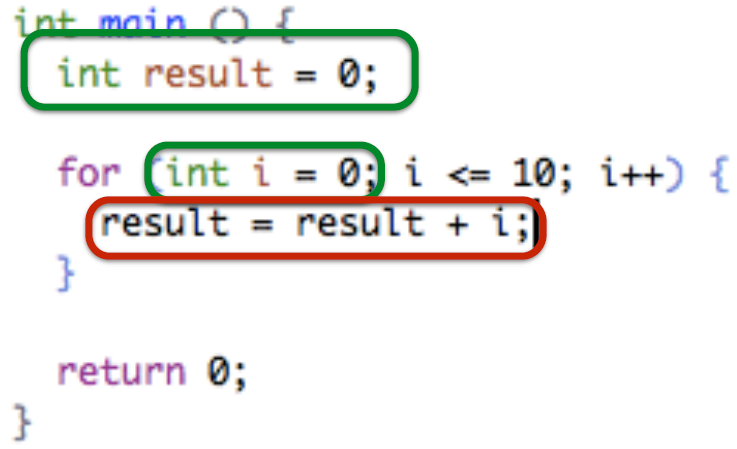
\includegraphics[width=.6\textwidth]{./image/cap5/bindings-C}
            \end{center}
        \end{itemize}
        \item<3-> Los lenguajes de máquina no utilizan identificadores, ergo bindings.
    \end{itemize}
\end{frame}

\begin{frame}{Tiempo de asociación}
    \begin{itemize}
        \item<1-> El \blue{tiempo} (o \blue{instante}) \blue{de asociación} (o \blue{ligado}), en inglés \blue{binding time}, es el momento en el cual una asociación es creada.
        \item<2-> Más en general, es el momento en que se toma una\\ \redb{decisión sobre implementación}.
        \item<3-> Puede ser:
        \begin{itemize}
            \item En tiempo de diseño
            \item En tiempo de implementación
            \item En tiempo de carga
            \item En tiempo de ejecución
        \end{itemize}
    \end{itemize}
\end{frame}

\begin{frame}{Tiempo de asociación}
    \begin{itemize}
        \item<1-> \blue{Al diseñar un lenguaje}: en la mayoría de los lenguajes, los datos y estructuras de control primitivas, así como otros muchos aspectos semánticos, se escogen al momento de diseñar el lenguaje.
        \item<2-> \blue{Al implementar un lenguaje}: típicamente las especificaciones de lenguajes dejan abiertas diversas decisiones de implementación. Ej: manejo de memoria, manejo de I/O, interacción con el sistema operativo, etc.
    \end{itemize}
\end{frame}

\begin{frame}{Tiempo de asociación}
    \begin{itemize}
        \item<1-> \blue{En tiempo de carga} (\blue{load time}): momento en que el sistema operativo carga el programa en memoria para ejecutarlo. Aquí se decide en qué ubicaciones de memoria reales se ejecutará.
        \begin{itemize}
            \item<2-> Análogamente, en la JVM los \redb{classloaders} permiten cargar una clase dinámicamente desde memoria.
        \end{itemize}
        \item<3-> \blue{En tiempo de ejecución}: aquí se asocian los \redb{valores} a identificadores o variables. Las bindings en tiempo de ejecución se denominan \redb{dinámicas}, en oposición a las \redb{estáticas}, que son todas las asociaciones hechas antes de la ejecución.
        \begin{itemize}
            \item<4-> Ej: en C++ las funciones \redb{virtual} son resueltas en tiempo de ejecución, mientras que las otras son resueltas en tiempo de compilación ({\em dynamic dispatch} en polimorfismos de POO)...
        \end{itemize}
    \end{itemize}
\end{frame}

\begin{frame}{}
    \begin{center}
        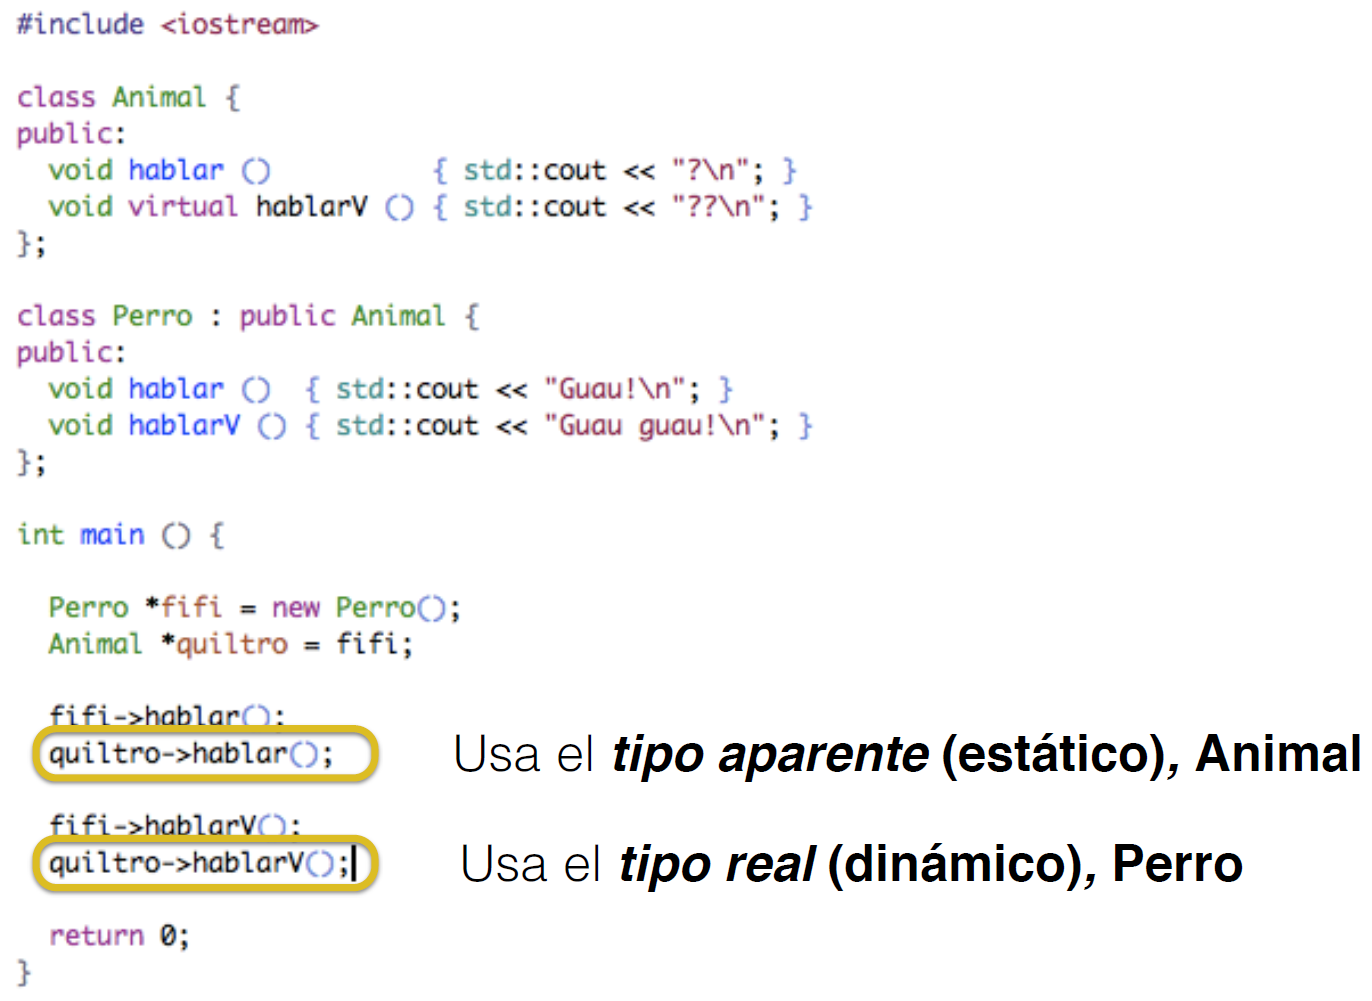
\includegraphics[width=\textwidth]{./image/cap5/ex-virtual}
    \end{center}
\end{frame}

\begin{frame}{Definición de los tiempos de asociación}
    \begin{itemize}
        \item Es una práctica crucial para el diseño e implementación de un lenguaje.
        \item En general tenemos que:
        \begin{itemize}
            \item mientras más ``temprano'' es la asociación, es posible obtener mayor \redb{eficiencia};
            \item mientras más ``tarde'' es la asociación, es posible obtener mayor \redb{flexibilidad}.
        \end{itemize}
    \end{itemize}
\end{frame}

%==============================
\section{Ámbito (Scope)}

\begin{frame}{Scope}
    \begin{itemize}
        \item<1-> Vimos que un \blue{binding} es la asociación de un nombre a una entidad.
        \item<2-> El \blue{scope} (o \blue{ámbito}) de un binding se refiere al ``alcance'' o parte del programa donde el binding es válido o activo.
        \item<3-> Un error típico de compilación:\\
        \red{\texttt{error: 'foo' was not declared in this scope}}
        \begin{flushright}
           {\small (veamos un ejemplo...)}
        \end{flushright}
        \item<4-> Fuera de su scope, el mismo nombre puede asociarse a otra entidad, usando un binding diferente.
    \end{itemize}
\end{frame}

\begin{frame}{Scope}
    \begin{itemize}
        \item<1-> Un poco imprecisamente, se entiende también \blue{scope} por un \blue{bloque de código}.
        \begin{itemize}
            \item Ej: En la familia C, delimitados por \texttt{$\{$} y \texttt{$\}$}.
            \item Ej: En la familia ALGOL, delimitados por \texttt{begin} y \texttt{end}.
        \end{itemize}
        \item<2-> El problema de determinar el scope de un binding es independiente de si el lenguaje es interpretado o compilado, o si tiene tipos estáticos o dinámicos.
        \item<3-> Existen dos grandes clasificaciones:
        \begin{itemize}
            \item \blue{Scope léxico} (o estático)
            \item \blue{Scope dinámico}
        \end{itemize}
    \end{itemize}
\end{frame}

%------------------------------
\subsection{Scope léxico}

\begin{frame}{Scope}
    \begin{itemize}
        \item<1-> Presente en la mayoría de lenguajes de programación.
        \item<1-> Los bindings pueden determinarse estáticamente por el compilador simplemente examinando el texto del programa.
        \item<2-> Para cualquier nombre, el binding activo asociado corresponde a la instancia de asociación léxicamente más cercana al uso del nombre.
    \end{itemize}
\end{frame}

\begin{frame}{Ejemplo: ¿Qué valor retorna?}
    \begin{center}
        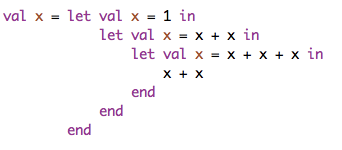
\includegraphics[width=.9\textwidth]{./image/cap5/scope01}
    \end{center}
\end{frame}

\begin{frame}{Solución 1: Substitución}
    \begin{center}
        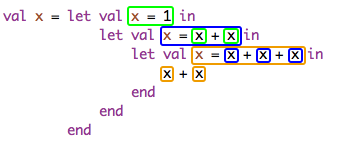
\includegraphics[width=.9\textwidth]{./image/cap5/scope02}
    \end{center}
\end{frame}

\begin{frame}{Solución 1: Substitución}
    \begin{center}
        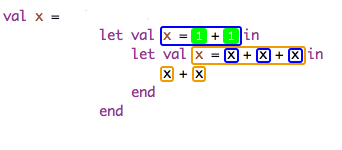
\includegraphics[width=.9\textwidth]{./image/cap5/scope03}
    \end{center}
\end{frame}

\begin{frame}{Solución 1: Substitución}
    \begin{center}
        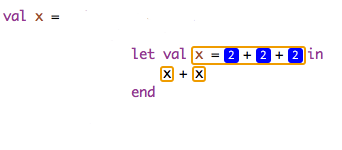
\includegraphics[width=.9\textwidth]{./image/cap5/scope04}
    \end{center}
\end{frame}

\begin{frame}{Solución 1: Substitución}
    \begin{center}
        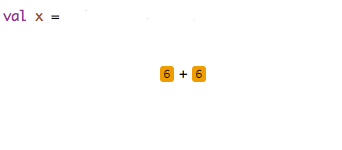
\includegraphics[width=.9\textwidth]{./image/cap5/scope05}
    \end{center}
\end{frame}

\begin{frame}{Solución 1: Substitución}
    \begin{center}
        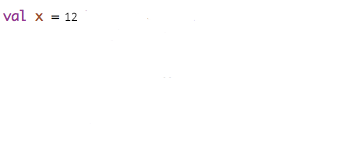
\includegraphics[width=.9\textwidth]{./image/cap5/scope06}
    \end{center}
\end{frame}

\begin{frame}{Substitución}
    \begin{itemize}
        \item<1-> La substitución es un método ineficiente.
        \begin{itemize}
            \item requiere inspeccionar todo el \blue{árbol de sintáxis}, incluso cuando el identificador no se usa.
        \end{itemize}
        \item<2-> Solución: usar una pila, conocida como el \blue{ambiente} o \blue{tabla de símbolos}.
        \item<2-> Esta estructura almacena las asociaciones nombre-valor de forma anidada, para respetar el scope léxico.
        \item<3-> Así, cuando se necesita conocer el valor de un nombre, se busca en el \blue{ambiente actual}.
    \end{itemize}
\end{frame}

\begin{frame}{Solución 2: Tabla de símbolos}
    \begin{center}
        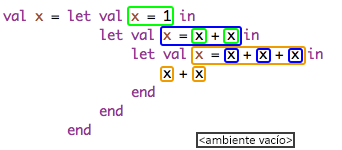
\includegraphics[width=.9\textwidth]{./image/cap5/scope-b02}
    \end{center}
\end{frame}

\begin{frame}{Solución 2: Tabla de símbolos}
    \begin{center}
        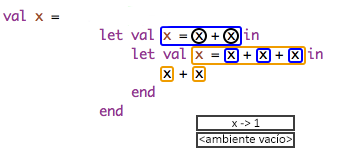
\includegraphics[width=.9\textwidth]{./image/cap5/scope-b03}
    \end{center}
\end{frame}

\begin{frame}{Solución 2: Tabla de símbolos}
    \begin{center}
        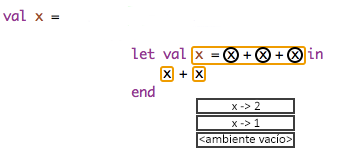
\includegraphics[width=.9\textwidth]{./image/cap5/scope-b04}
    \end{center}
\end{frame}

\begin{frame}{Solución 2: Tabla de símbolos}
    \begin{center}
        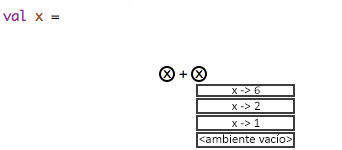
\includegraphics[width=.9\textwidth]{./image/cap5/scope-b05}
    \end{center}
\end{frame}

\begin{frame}{Solución 2: Tabla de símbolos}
    \begin{center}
        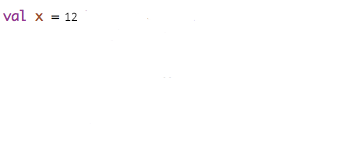
\includegraphics[width=.9\textwidth]{./image/cap5/scope06}
    \end{center}
\end{frame}

\begin{frame}{Scope en algunos lenguajes}
    \begin{itemize}
        \item En C tenemos el scope global, y los scopes locales de cada función. En general no hay \blue{scopes anidados} como los recién vistos en SML.
        \item En Java existe el scope de clase, de método, de package, y los scopes anidados (inner classes).
        \item En Javascript también existe un scope global, y scopes locales para cada función.
    \end{itemize}
\end{frame}

\begin{frame}{Scopes anidados}
    \begin{itemize}
        \item En general, cuando se tienen scopes anidados, es necesario decidir qué hacer cuando se repiten nombres de identificadores (como en el ejemplo).
        \item La regla general es que el scope más próximo ``oculta'' al más externo. Algunos lenguajes como Java permite acceder de todas maneras a la asociación exterior usando keywords como ``outer''.
        \begin{itemize}
            \item Buscar por \blue{nested classes}, \blue{inner class} y \blue{outer class}.
        \end{itemize}
    \end{itemize}
\end{frame}

\begin{frame}{Orden de declaraciones}
    \begin{itemize}
        \item<1-> El concepto de scope también considera cómo un lenguaje maneja el orden en que hacemos las declaraciones de variables u otras asociaciones.
        \item<2-> Si declaramos un objeto o valor \texttt{x} dentro de un bloque:
        \begin{itemize}
            \item ¿su alcance incluye las declaraciones anteriores del bloque?
            \item ¿o sólo desde su declaración hacia ``adelante''?
        \end{itemize}
        \item<3-> ¿Puede una declaración o expresión referirse a todos los nombres declarados en el scope actual, o sólo a aquellos declarados antes de dicha expresión?
    \end{itemize}
\end{frame}

\begin{frame}{Orden de declaraciones}
    \begin{center}
        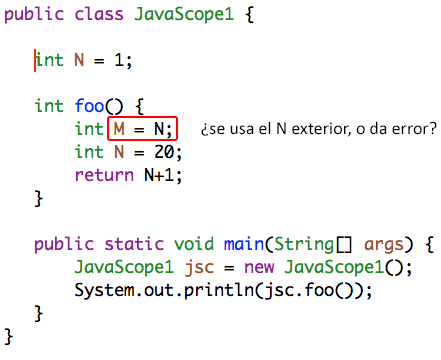
\includegraphics[width=.7\textwidth]{./image/cap5/scope-java}
    \end{center}
\end{frame}

\begin{frame}{Orden de declaraciones}
    \begin{center}
        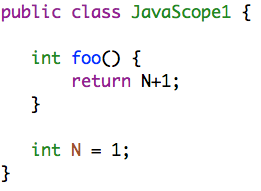
\includegraphics[width=.5\textwidth]{./image/cap5/scope-java2}
    \end{center}
    Una clase en Java puede acceder a sus variables de instancia desde cualquier método, sin importar el orden.
\end{frame}

\begin{frame}{Orden de declaraciones}
    Pero en C\# no es igual que en Java...
    \begin{center}
        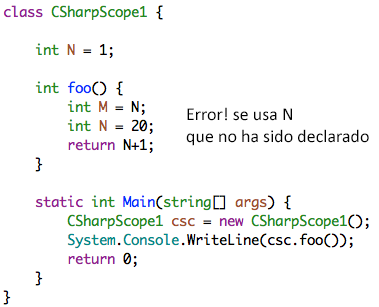
\includegraphics[width=.7\textwidth]{./image/cap5/scope-Csharp}
    \end{center}
\end{frame}

\begin{frame}{Orden de declaraciones}
    \begin{itemize}
        \item El comportamiento en C\# asume que la declaración local de \texttt{N} en el método \texttt{foo()} abarca todo el scope de dicho método; es decir, no acepta declaraciones externas.
        \item En otras palabras, la variable local \texttt{N} está ocultando la variable de instancia \texttt{N}. Esto es detectado por el compilador.
        \item Soluciones: renombrar la variable local, o usar \texttt{this.N} para referirse explícitamente a la variable de instancia.
    \end{itemize}
\end{frame}

\begin{frame}{Orden de declaraciones: otros enfoques}
    \begin{itemize}
        \item En Python es similar a C\#, pero las variables son ``declaradas'' cuando existe una asignación.
        \item SML y Racket usan variantes de \blue{\texttt{let}} para controlar de manera más precisa el alcance de las definiciones.
        \item En Modula-3 el alcance de una declaración es el bloque completo (sin contar bloques anidados), y no importa el orden de declaración.
    \end{itemize}
\end{frame}

\begin{frame}{Orden de declaraciones}
    \begin{center}
        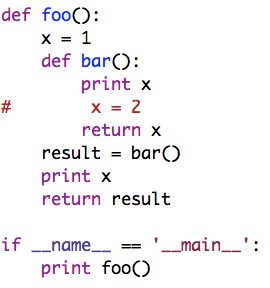
\includegraphics[width=.5\textwidth]{./image/cap5/scope-modula3}
    \end{center}
\end{frame}

\begin{frame}{Declaraciones y recursión}
    \begin{itemize}
        \item En estructuras o tipos mutuamente recursivos, es imposible que una declaración aparezca antes que la otra.
        \begin{itemize}
            \item Para ello es necesario soluciones adicionales.
        \end{itemize}
        \item En C y C++ se usa el concepto de {\em definición} o {\em prototipo}, que separa la declaración y la implementación de una estructura o función.
        \item En SML se ocupa la keyword \texttt{and} para definiciones mutuamente recursivas.
    \end{itemize}
\end{frame}

\begin{frame}{Declaraciones y recursión}
    \begin{center}
        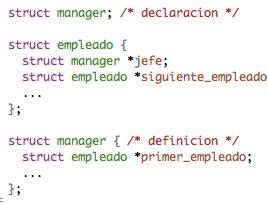
\includegraphics[width=.6\textwidth]{./image/cap5/scope-C-recursivo}
    \end{center}
\end{frame}

\begin{frame}{Declaraciones y recursión}
    \begin{center}
        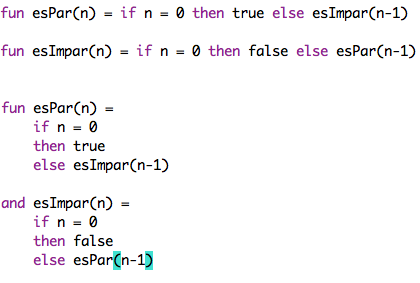
\includegraphics[width=.7\textwidth]{./image/cap5/scope-SML-recursivo}
    \end{center}
\end{frame}

\begin{frame}{Bloques anidados}
    \begin{itemize}
        \item Muchos lenguajes permiten declarar variables locales en bloques anidados, cuyo alcance está limitado exclusivamente a ese bloque.
        \item En general las declaraciones en un bloque anidado ocultan las del scope exterior.
        \item El uso de bloques anidados puede facilitar la lectura del programa y eliminar la posibilidad de interferir accidentalmente con otras variables del mismo nombre.
    \end{itemize}
\end{frame}

\begin{frame}{Bloques anidados}
    \begin{center}
        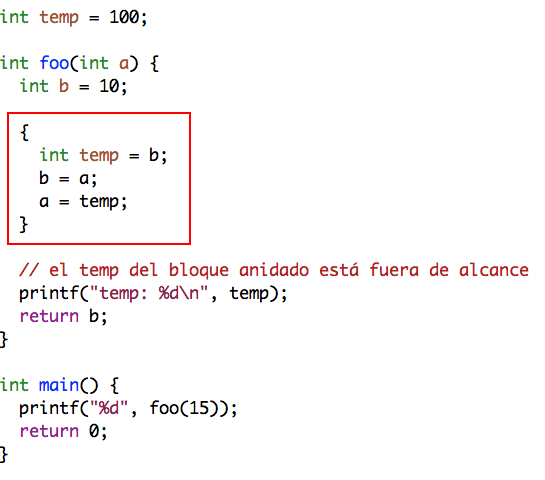
\includegraphics[width=.8\textwidth]{./image/cap5/scope-bloques-anidados}
    \end{center}
\end{frame}

%------------------------------
\subsection{Scope dinámico}

\begin{frame}{Scope dinámico}
    \begin{itemize}
        \item<1-> Los bindings dependen del flujo de control en tiempo de ejecución; especialmente en el orden en que las funciones o subrutinas son llamadas.
        \item<2-> El binding activo para un nombre es el \redb{más reciente durante la ejecución}.
        \item<3-> Ej: El lenguaje de scripting BASH tiene scope dinámico.
    \end{itemize}
\end{frame}

\begin{frame}{Ejemplo: Scope dinámico en Bash}
    \begin{center}
        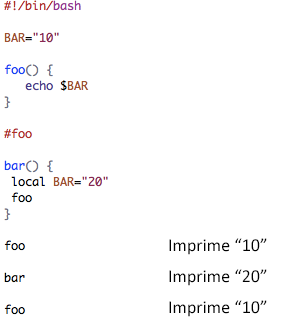
\includegraphics[width=.6\textwidth]{./image/cap5/scope-bash}
    \end{center}
\end{frame}

\begin{frame}{Ventajas y desventajas}
    \begin{itemize}
        \item<1-> El uso indiscriminado de scope dinámico puede llevar a errores de ejecución difíciles de identificar.
        \begin{itemize}
            \item Es necesario conocer todos los nombres de identificadores ya definidos con los cuales pueden existir conflictos.
        \end{itemize}
        \item<2-> Las funciones que usan identificadores con scope dinámico son más fáciles de personalizar.
        \item<3-> Actualmente se considera al scope léxico como mejor opción por defecto.
        \begin{itemize}
            \item Algunos lenguajes usan mecanismos específicos y acotados para introducir scope dinámico.
        \end{itemize}
    \end{itemize}
\end{frame}

%------------------------------

\begin{frame}
 \begin{block}{Bibliografía}
  \begin{itemize}
    \item Pratt, Terrence W. (1998). \textit{Lenguajes de programación: diseño e implementación}, Pearson Education.
    \item Sethi, Ravi (1992). \textit{Lenguajes de programación: conceptos y constructores}, Addison-Wesley Iberoamericana.
    \item Scott, Michael (2009). \textit{Programming Language Pragmatics}, Morgan Kaufman, 3ra ed.
  \end{itemize}
 \end{block}
 \begin{block}{Recursos}
  \begin{itemize}
    \item Apuntes de cursos anteriores (Ismael Figueroa).
    \item Wikipedia y Wikimedia Commons.
    \item Imágenes con licencia libre.
  \end{itemize}
 \end{block}
\end{frame}

\end{document}
